\section{Orientation Recovery}
\label{sec:orientation-recovery}

Equipped with an appropriately learned $\widehat{d}_b$, the objective is then to recover the unknown unit quaternions $\big\{q_p\big\}_{p=1}^P$ associated to the projections $\big\{\mathbf{b}^p\big\}_{p=1}^P$ in any given dataset.

% ----------------------------------------------------
\subsection{Minimization Scheme}

We propose to start this process by computing of a great number of pairwise projection distances $\big\{\widehat{d}_b\big(\mathbf{b}^i,\mathbf{b}^j\big)\big\}_{i,j=1}^{P}$ through $\widehat{d}_b$. Then, our postulate is that we can recover the orientations from theses distances by solving
%---
\begin{equation}
    \label{eq:global-min-problem}
    \big\{\widehat{q}_p\big\}_{p=1}^P=\argmin{q_i\in\mathbb{U}}\sum_{i,j} \big|\widehat{d}_b\big(\mathbf{b}^i,\mathbf{b}^j\big) - d_q\big(q_i,q_j\big) \big|^2,
\end{equation}
% ---
as is illustrated in Figure~\ref{fig:overview-pipeline}.

In practice, one cannot possibly evaluate~\eqref{eq:global-min-problem} for every pair of orientations $\big\{q_i,q_j\big\}_{i,j=1}^P$ given the extremely large size of SPA datasets, with $P$ typically in the order of dozens of thousands. Hence, we need to partially sample the projection dataset. We experimentally demonstrate in Section~\ref{subsec:5-6-3-sanity-check} that this does not affect the performance of our recovery scheme.

As previously discussed, we are not yet aware of any guarantee of convergence for~\eqref{eq:global-min-problem}. Similarly, we do not know of any theoretical characterization of the behaviour of~\eqref{eq:global-min-problem} in ill-posed conditions, such as when pairwise distances are misestimated, for instance. Hence, we rely for now on experimental demonstrations to 1) ensure feasibility, and 2) indicate where efforts need to be invested.

% ----
\begin{figure}[t]
    \centering
    \begin{subfigure}[b]{0.48\textwidth}
        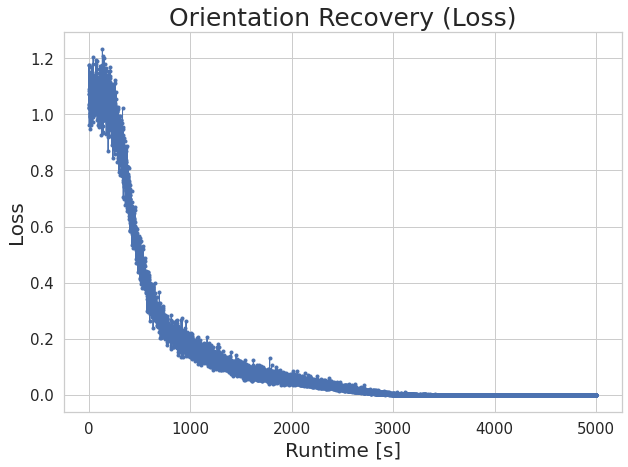
\includegraphics[width=\textwidth]{fig_perfectdistances_loss-symmetric.png}
        \caption{}
    \end{subfigure} \quad
    \begin{subfigure}[b]{0.48\textwidth}
    \centering
        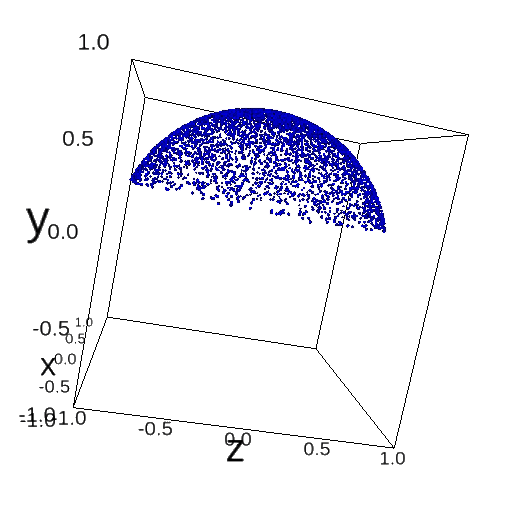
\includegraphics[width=0.8\textwidth]{fig-perfectdistances-coverage-symmetric.png}
        \caption{}
    \end{subfigure}
    \caption{Results of the orientation recovery scheme when using the perfect orientation distances for the asymmetric protein (5j0n). \textbf{(a)} Evolution of the loss of~\eqref{eq:global-min-problem} during minimization. \textbf{(b)} Coverage of $\SOThree$ after the orientation recovery from the perfect relative distances. }
    \label{fig:minim-loss-perfect-distances}
\end{figure}
% ---

% ----------------------------------------------------
\subsection{Feasibility Check: Recovery from the Exact Relative Distances}
\label{subsec:5-6-3-sanity-check}

Our first investigation is to verify that it is at all possible to recover the orientations through~\eqref{eq:global-min-problem} from their true relative distances (\textit{i.e.}, using $d_q$ and not a proxy $d_b$).

We use the $5,000$ projections from the asymmetric protein (5j0n) dataset. Out of the possible 25 mio possible pairs, we randomly select only $5,000$ of them and compute their geodesic distance through~\eqref{eq:geodesic distance}. We then minimize~\eqref{eq:global-min-problem} using the SGD Adam optimizer~\cite{kingma2014adam} for $30K$ steps ($\sim$1 hour) with a learning rate of $0.1$.

The results are given in Figure~\ref{fig:minim-loss-perfect-distances}. They confirm that it is possible to recover the orientations from their true relative distances, even though the embedding space is non-Euclidean. As previously discussed, this is not a straightforward result. The results also demonstrate that a large subsampling of the projection pairs does not affect the convergence of~\eqref{eq:global-min-problem}, which is in straight line with the observations made by numerous Euclidean-based dimensionality reduction works~\cite{belkin2003laplacian,kruskal1978multidimensional, maaten2008visualizing, mcinnes2018umap}.

% ----------------------------------------------------
\subsection{Robustness of Recovery to Additive Errors on the Relative Distances}
\label{subsec:5-6-4-robustness-to-errors}

We now go one step further and evaluate the behaviour of~\eqref{eq:global-min-problem} when the true relative distances are corrupted by  additive Gaussian noise.

The experimental conditions are the same than in the previous section, except that we add an error with increasing variance on the relative distances prior to the minimization. The results are presented in Figure~\ref{fig:recovery-noise-distances} (red curve).

% ----
\begin{figure}
    \centering
    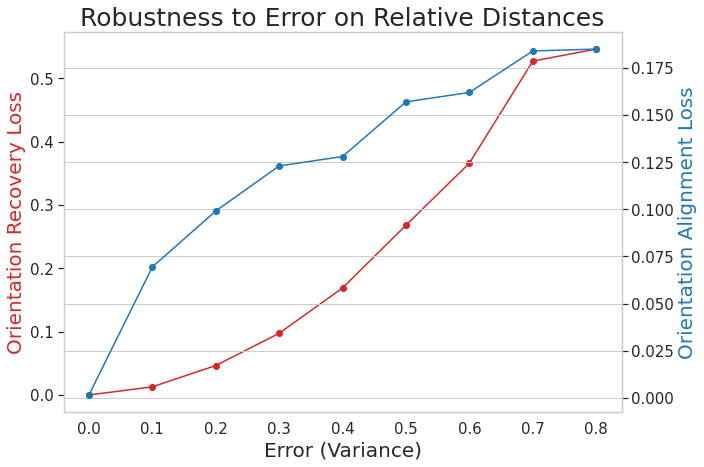
\includegraphics[width=0.75\textwidth]{fig-robustness-asymmetric.png}
    \caption{Results of the recovery scheme (red curve) and the alignment procedure (blue curve) when an increasing amount of errors is added to the true relative distances.}
    \label{fig:recovery-noise-distances}
\end{figure}
% ---

Before discussing the results, we remark that one cannot really quantify the performance of~\eqref{eq:global-min-problem} through its loss. Unfortunately, it is also not appropriate to directly compute the error between the recovered orientations $\big\{\widehat{q}_p\big\}_{p=1}^P$ and the true ones $\big\{q_p\big\}_{p=1}^P$. The reason is that the recovery of orientation through~\eqref{eq:global-min-problem} is up to a global rotation, \textit{i.e.}, any global rotation of the set of recovered orientations is as valid as any other. This is not a problem for the ultimate application of our scheme, but it complicates the quantitative evaluation of its performance in synthetic experiments. We circumvent this problem by 1) aligning the true and recovered orientation sets, and 2) computing their distance after alignment. The alignment is performed by searching for the orthogonal matrix (with determinant $\pm$ 1) $\mathbf{T}\in\mathbb{R}^4$  that minimizes
% ---
\begin{equation}
    \label{eq:alignement}
    \widehat{\mathbf{T}}=\argmin{\mathbf{T}\in\mathbb{R}^4}\sum_{i,j} \big|d_q\big(q_i,q_j\big)- d_q\big(\mathbf{T}\widehat{q}_i,\mathbf{T}\widehat{q}_j\big)\big|^2.
\end{equation}
% ---
For all variances, the distance after alignment is reported in Figure~\ref{fig:recovery-noise-distances} (blue curve).

These results demonstrate that the performance of the minimization scheme~\eqref{eq:global-min-problem} linearly depends on the quality of the relative distances, which advocates for a proper and extensive training of the SiameseNN in the next stages of development. Another interesting output of Figure~\ref{fig:recovery-noise-distances} is that it indicates that the error of the orientation recovery behaves as a monotonic function of its loss. Hence, it suggests that the loss can be used as a good indicator of its performance, which has obvious practical implications for our future works on real data.
